\documentclass[a4paper]{report}
\usepackage[T1]{fontenc}
\usepackage[utf8]{inputenc}
\usepackage[english]{babel}
\usepackage{titlesec}
\usepackage{lipsum}
\usepackage{booktabs}
\usepackage{hyperref}
\usepackage{graphicx}
\usepackage{float}
\usepackage{rotating}
\usepackage[dvipsnames]{xcolor}
\usepackage{enumerate}
\usepackage[shortlabels]{enumitem}
\usepackage{geometry}
\usepackage{pdflscape}
\usepackage{caption}
\graphicspath{{./img/}}

\begin{document}

%%The two following lines remove the line "Chapter n" at the beginning of each chapter, before the title
%\titleformat{\chapter}[display]
%  {\normalfont\bfseries}{}{0pt}{\Large}
\titleformat{\chapter}[hang] 
{\normalfont\huge\bfseries}{\thechapter}{1em}{} 

\title{SafeStreets}
\author{Rosetti Nicola, Sartoni Simone, Torri Vittorio}
\date{date} %%TODO

\begin{titlepage}
\begin{figure}[t]
\centering
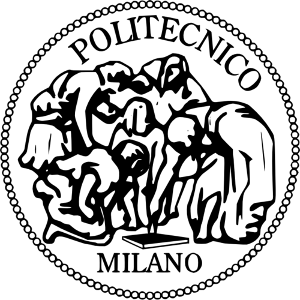
\includegraphics[width=0.3\textwidth]{Logo}
\end{figure}
\begin{center}
    \textsc{ \LARGE{Politecnico di Milano \\}}
	\textsc{ \Large {School of Industrial and Information Engineering\\ }}
	\textnormal{ \Large{Master of Science in Computer Science and Engineering\\}}
	\vspace{3mm}
	\textnormal{ \Large{Software Engineering 2 Mandatory Project\\}}
	\vspace{30mm}
	\fontsize{10mm}{7mm}\selectfont 
    \textup{Safe Streets.}\\
    \textnormal{ \LARGE{Design Document\\}}
\end{center}

\vspace{18mm}

\begin{center}
    \textnormal{\large{\bf Authors:\\}}
	{\large Rosetti Nicola \\ Sartoni Simone \\ Torri Vittorio }
	\fontsize{10mm}{5mm}\selectfont 
\end{center}
\vspace{15mm}

\centering{\large{
Academic Year 2019/2020 \\
\vspace{10mm}
Milano, 09/12/2019 \\
\vspace{2mm}
Version 1.0 
}}

\end{titlepage}

\newgeometry{top=3cm}
\tableofcontents
\listoffigures
\begingroup
\let\clearpage\relax %avoid to put it on a new page
\listoftables
\endgroup
\restoregeometry

\chapter{Introduction}
\section{Purpose}
\section{Scope}
\section{Definitions,Acronyms,Abbreviations}
\section{Revision History}
\section{Reference Documents}
\section{Document Structure}

\chapter{Architectural Design}
\section{Overview: High­‐level components and their	interaction}
The application will be developed using the client-server paradigm on a three-tiered architecture. The three layers of the application (Presentation, Application and Data) are divided into clusters of machines (i.e. tiers) that actually cooperate to provide a specific functionality. In this case we have three tiers  and each tier is responsible for one of the three layers. The client side is responsible (only) for the presentation layer; therefore, in this architecture, the thin-client has been adopted considering the fact that the required functionalities client-side are limited. The UIs provided are just meant to show results and to allow clients to choose what they want.  In the App case, the client contains all the presentation layer while in the WebApp case the layer is splitted between the client and WebServer; the WebServer is responsible for contacting the application server and forward the client requests to it. The Application tier takes care of the application layer encapsulating all is needed concerning the application logic. It receives the requests from the clients and handles them. It's also responsible for sending asynchronous notifications to the presentation layer when certain conditions are met.  Here we have multiple Servers cooperating together to improve performance, scalability, fault tolerance and availability. An elastic component (i.e. load balancer) is used to rule the accesses to different Application Servers, dinamically balancing the load among all the Servers. The Application tier communicates with the Data tier, responsible for the Data Access layer. This tier is composed by several DataServers: each one is associated with a single replica of the data and exploits the DBMS technology to access the DataBase. The Database is fully replicated in different nodes. Techniques and protocols are used to ensure consistency among replicas: they will be full explained in "Other design decisions" section. Again a load balancer is used to dinamically share the load among different machines. 
To ensure and improve security firewalls are installed before and after the application servers to filter accesses from external and unsafe networks. By the creation of a DMZ (demilitarized zone) external entities can only have access to the exposed services. Security is crucial because the application works mainly with sensible information.
To provide the required functionalities the system exploits datawarehousing. The datawarehouse is a component in the Data tier able to deal with historical data and aggregate data taken from the Databases exploiting data mining technologies to answer complex queries: used techniques are clustering, associative rules and classification. This component periodically queries one dataServer to retrieve new information and updates on the data since its last update. 
\section{Component view}
In the figure \ref{fig:component-diagram} is reported the \textit{Component Diagram} for the SafeStreet system. This is a high level view in which the main components are shown, then some components will be better detailed.

\newgeometry{bottom=2cm}
\begin{landscape}

\begin{figure}[hp]
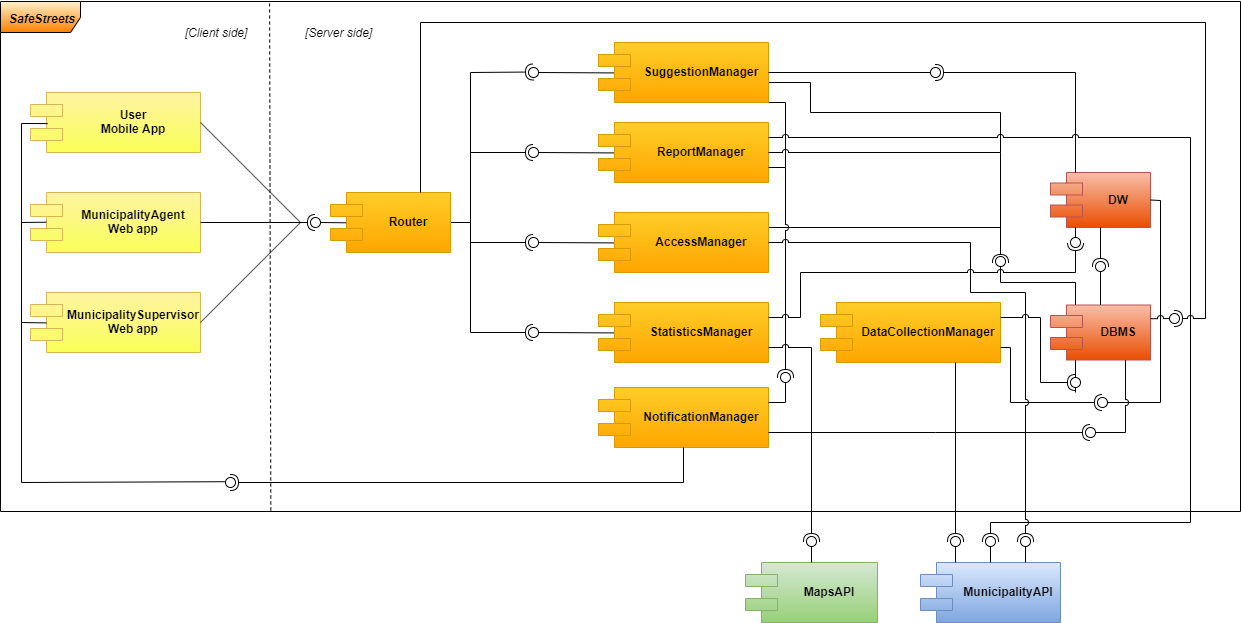
\includegraphics[angle=0, scale=0.55]{Component1}
\caption{UML Component Diagram}
\label{fig:component-diagram}
\end{figure}

\end{landscape}
\restoregeometry
In this diagram when two components can communicate using different interfaces a single interface link is 
reported, for the sake of readability. The various components are now described and detailed:
\begin{itemize}
\item \textbf{Router}: it has the role of dispatching the requests coming from the users applications. Before doing this it has also the important role of verifying the user authentication, checking the token which is sent with all requests performed by an authenticated user. In figure \ref{fig:router-component} a more detailed view is provided, putting in evidence the various interfaces for the mobile and for the web app.
\begin{figure}[hp]
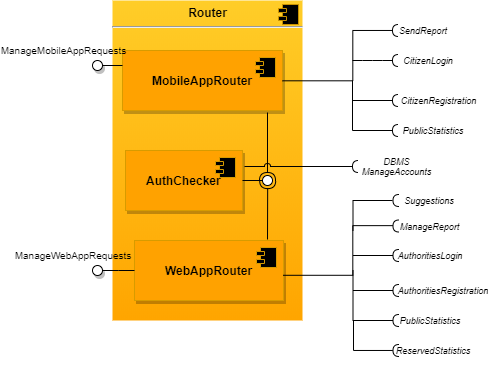
\includegraphics[width=\textwidth]{Router}
\caption{UML Component Diagram for \textit{Router} component}
\label{fig:router-component}
\end{figure}
\item \textbf{SuggestionsManager} this components is the one which elaborates and provides the \textit{Suggestions} for the municipalities. It analyzes the data exploiting the \textit{DataWarehouse} component for the aggregated queries about reports, accidents and tickets and the \textit{DBMS Component} to retrieve non-aggregated information about the streets. It can provide the actual available suggestions for a municipality as an answer to a request coming from the \textit{Router}, but it also notify the \textit{Municipality Supervisor web app} through the \textit{NotificationManager} component when it discovers a new suggestion (the suggestion discover task is periodically executed, once a month).
\item \textbf{ReportManager}: this component is in charge of all concern the management of the reports sent by the users. It receives them by the mobile application and execute the automatic analysis to identify possible fake reports, it stores them through the \textit{DBMS Component} and it provides the reports to the the \textit{Municipality Agents web app}, answering to their requests of confirm/enqueue/discard and allowing them to emit a ticket, exploiting the \textit{Municipality APIs} which provide an interface for this service. Its detailed diagram is shown in figure \ref{fig:reportmgr-component}.

\begin{figure}[htp]
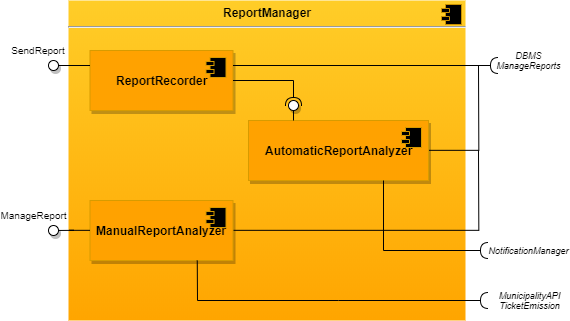
\includegraphics[width=\textwidth]{ReportManager}
\caption{UML Component Diagram for \textit{ReportManager} component}
\label{fig:reportmgr-component}
\end{figure}

\item \textbf{AccessManager}: it manages everything about registration and login of the users. For the citizens registration it calls the municipality service for the verification of identity cards, while for the agents and supervisors registration it calls the municipality service for their identity verification. He stores the accounts data through the \textit{DBMS} component and it calls it also to verify the correctness of the login credentials. Once a login has been correctly performed it generates a token, stored in the database and sent back to the user, necessary to perform authenticated requests. This component is detailed in figure \ref{fig:accessmgr-component}.

\begin{figure}[htp]
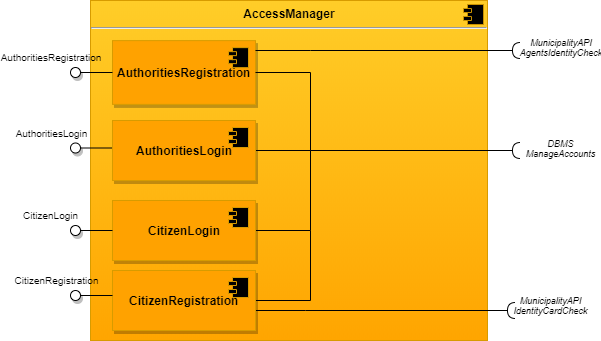
\includegraphics[width=\textwidth]{AccessManager}
\caption{UML Component Diagram for \textit{AccessManager} component}
\label{fig:accessmgr-component}
\end{figure}

\item \textbf{StatisticsManager}: it answers to the statistics requests, both public and reserved, and in doing this it calls the \textit{DataWarehouse} component. It is shown in the diagram in figure \ref{fig:statisticsmgr-component}.

\begin{figure}[htp]
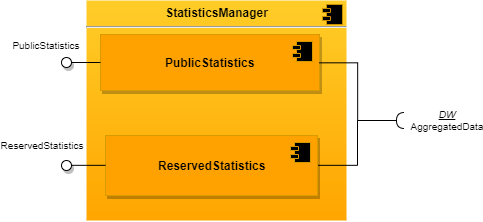
\includegraphics[width=\textwidth]{StatisticsManager}
\caption{UML Component Diagram for \textit{StatisticsManager} component}
\label{fig:statisticsmgr-component}
\end{figure}

\item \textbf{NotificationManager}: this component is the one able to send push notifications to the user clients, both mobile apps and web apps. It is exploited by the \textit{SuggestionManager} and by the \textit{ReportManager}.

\item \textbf{DataCollectionManager}: this component periodically retrieves the data made available by the municipality about accidents, tickets and street characteristics. These latter are store in the operational database, while the others are retrieved as aggregated data and so are directly stored in the datawarehouse.

\begin{figure}[htp]
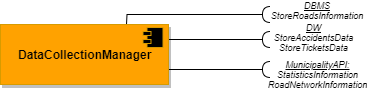
\includegraphics[width=\textwidth]{DataCollectionManager2}
\caption{UML Component Diagram for \textit{DataCollectionManager} component}
\label{fig:statisticsmgr-component}
\end{figure}

\item \textbf{DBMS}: this component manages the operational database, the main base for the functions of SafeStreets, being in charge of reports, users and streets data.

\item \textbf{DataWarehouse}: this component manages the datawarehouse, the secondary database for the system, used to answer aggregate queries for statistics and suggestions. It is periodically alimented with the dbms data and with the already aggregated data coming from the municipality through the \textit{DataCollectionManager} component.

\item \textbf{MunicipalityAPI}: this is an external component, managed by the municipalities (an instance for each of them which supports the system), whose interface is standardized as described in the \textit{Components Interfaces} section. It is necessary to retrieve the data for building statistics and suggestions and to have the possibility of traffic ticket emission through SafeStreets.

\item \textbf{MapsAPI}: this is an external component which is exploited to show maps with the statistics data.

\item \textbf{UserMobileApp}: this component entirely resides in the \textit{Presentation layer} and it's just an interface to allow the users to use SafeStreets on their mobile devices, sending reports and retrieving statistics information. It performs only minimal controls on the forms before sending them (ex: they are not missing mandatory field).

\item \textbf{AgentWebApp}: this component is the \textit{Presentation layer} of the web app which allows agents to see the reports, analyze them, emit tickets and retrieve users data.

\item \textbf{SupervisorWebApp}: this component is the \textit{Presentation layer} of the web app which allows supervisors to see the reports, possibly analyze them, retrieve all type of statistics and receive the suggestions elaborated by the system. 



\end{itemize}

\section{Deployment view}

\section{Runtime view}
In the figures \ref{fig:seq-sendReport}, \ref{fig:seq-userLogin}, \ref{fig:seq-checkReport}, \ref{fig:seq-checkStats}, \ref{fig:seq-register} and \ref{fig:seq-suggestions} some architectural sequence diagrams are provided, showing the interactions among the different components in the execution of various functions of the systems. \\
The only methods present here and not mentioned in the \textit{Component Intefaces} section are internal method of a single component.
\subsection{User sends a Report}
\newgeometry{left=0.5cm, bottom=2cm}
\begin{landscape}

\begin{figure}[hp]
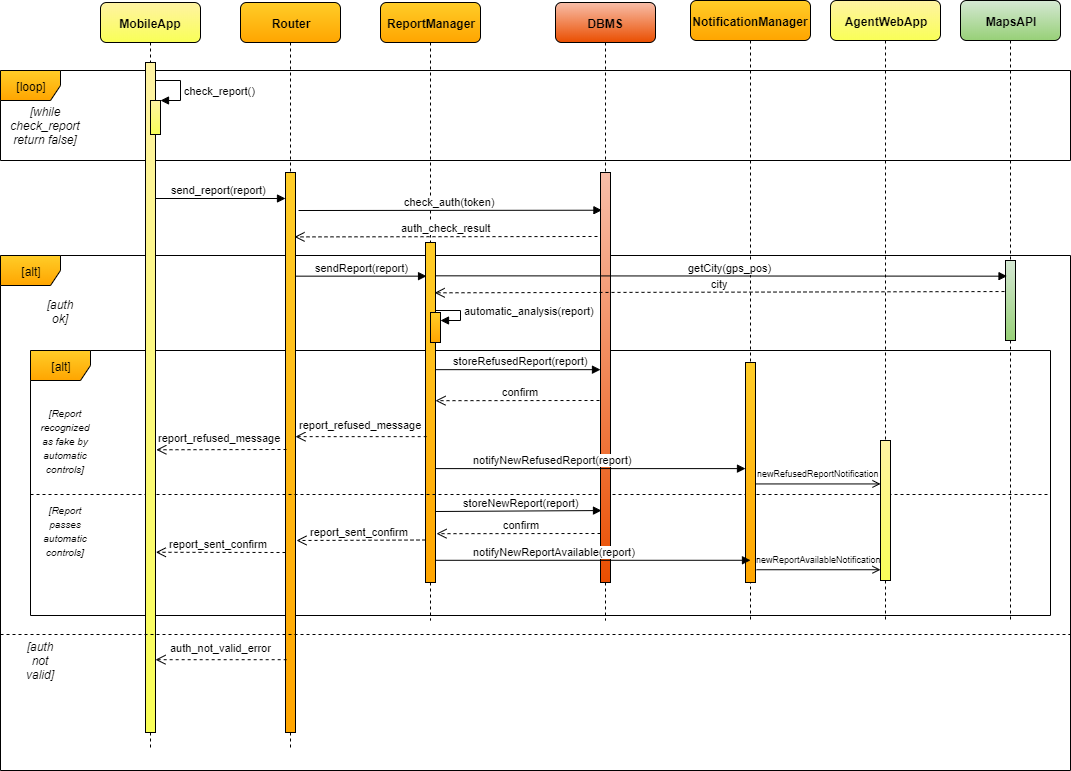
\includegraphics[angle=0, scale=0.70]{ArchSequenceSendReport}
\caption{UML Architectural Sequence Diagram for \textit{SendReport} use case}
\label{fig:seq-sendReport}
\end{figure}

\end{landscape}
\restoregeometry

In this sequence diagram is shown what messages are actually exchanged among components to process correctly a report send by a User. The User, through the Mobile App, fills the report form and sends it to the server for a confirm. The report is handled at first by the Router that checks if the User can actually send reports (i.e. verifies if the corresponding token has the rights needed). if the check is negative, then the request is discarded. Otherwise the ReportManager contacts the MapsAPI to retrieve the municipality in charge for a specific report. After this, the ReportManager checks internally if the pictures in the report have been modified or not. If so, the report is stored as "Refused" and sent to the Notification Manager, that will send a notification about the refused report to the involved MunicipalityAgent Web App. If the pictures are not fake then the report is stored as New report and the NotificationManager will be in charge of notifying the Municipality Web App about the new pending report.
  
\subsection{User Logs in}
\begin{landscape}

\begin{figure}[hp]
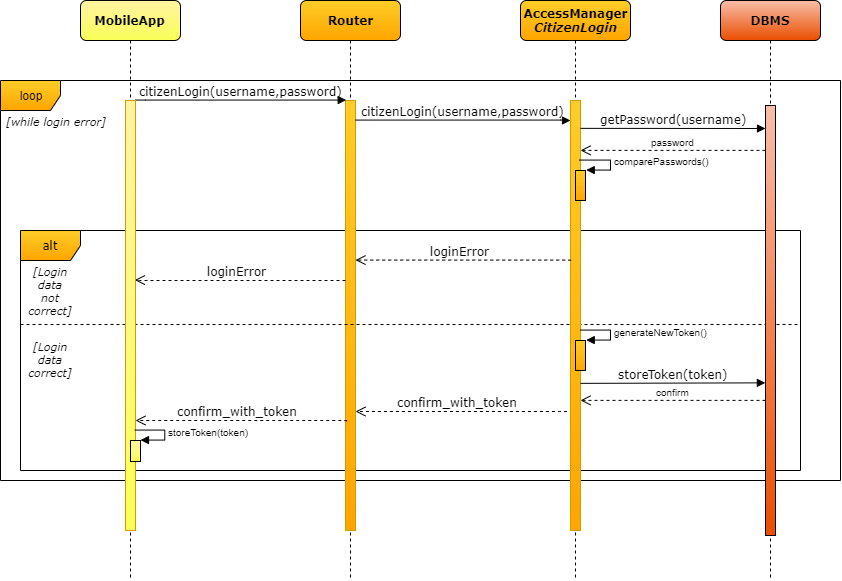
\includegraphics[angle=0, scale=0.70]{ArchSequenceUserLogin}
\caption{UML Architectural Sequence Diagram for \textit{UserLogin} use case}
\label{fig:seq-userLogin}
\end{figure}

\end{landscape}
\subsection{Agent Checks Report}
\newgeometry{left=0.5cm,right=0.5cm,bottom=3cm}
\begin{figure}[hp]
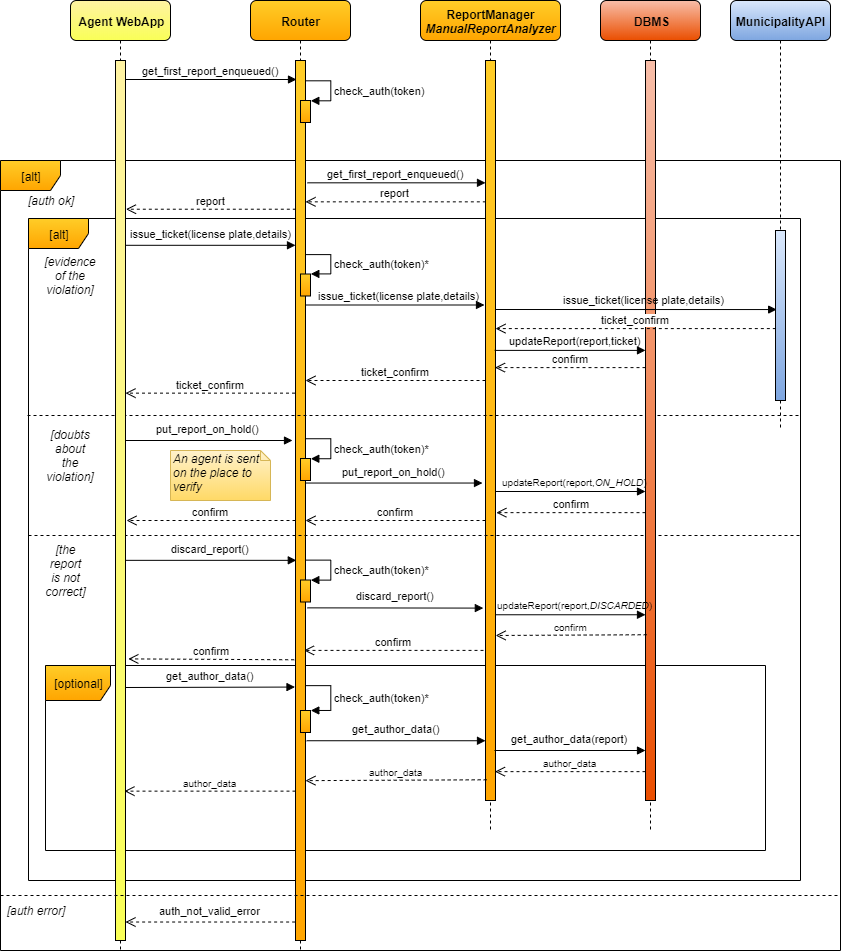
\includegraphics[width=\textwidth]{ArchSequenceAgentCheckReport}
\caption{UML Architectural Sequence Diagram for \textit{AgentCheckReport} use case}
\label{fig:seq-checkReport}
\end{figure}
\restoregeometry

In this sequence diagram are described the components involved i nthe user login and their interaction. The User fills the spaces in the Mobile App inserting his username and password. The login request is then sent to the Router that forwards the message to the AccessManager. In particular the subcomponent \textbf{CitizenLogin}  handles the login, asking the DB the password corresponding to the specified username. After having received the password, it internally checks if  the two passwords (the one coming from the user and the one stored)coincide: if so, the user is successfully logged in and this is notified back to the client, showing him the main page of the App; if not, a notification is sent back to the client, showing him an error message and asking him to insert again username and password. Notice that everytime a new login is performed a new token is generated associated to the specific logged client.

\subsection{Supervisor Checks Statistics}
\begin{landscape}

\begin{figure}[hp]
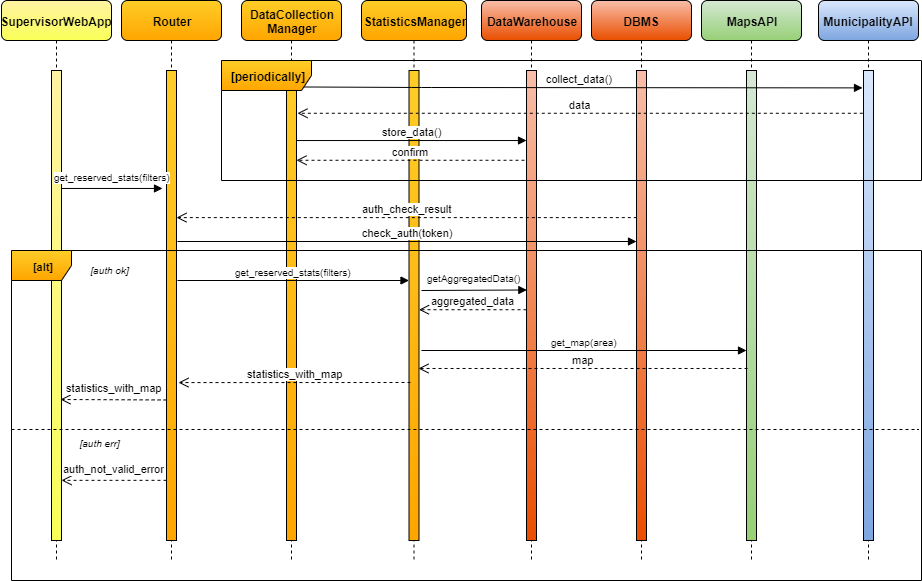
\includegraphics[angle=0, scale=0.70]{ArchSequenceCheckStatistics}
\caption{UML Architectural Sequence Diagram for the \textit{CheckStatistics} use case}
\label{fig:seq-checkStats}
\end{figure}

\end{landscape}

\newgeometry{left=0.5cm,right=0.5cm,bottom=3cm}
\begin{figure}[hp]
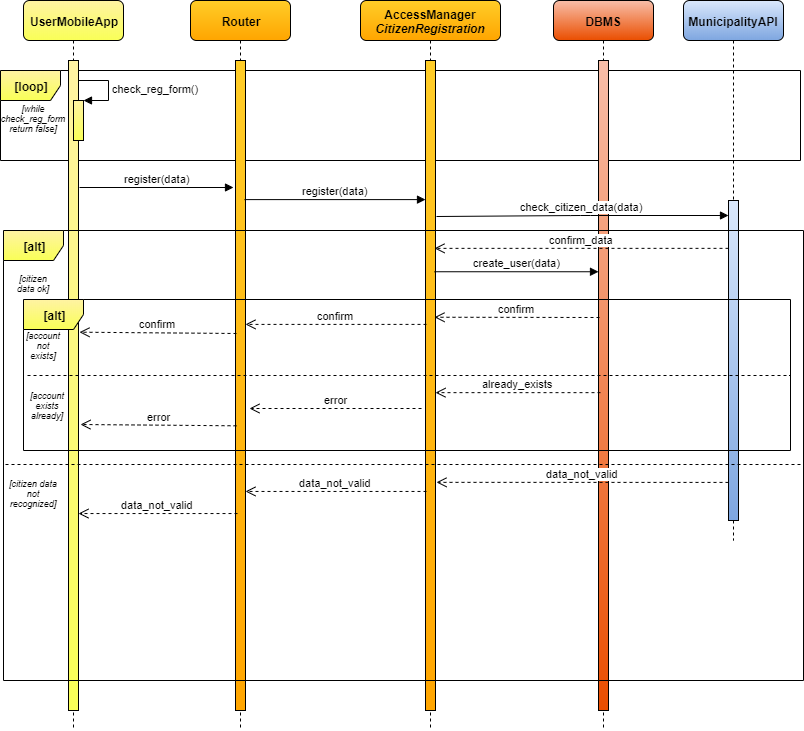
\includegraphics[scale=0.7]{ArchSequenceRegistration}
\caption{UML Architectural Sequence Diagram for \textit{User Registration}}
\label{fig:seq-register}
\end{figure}
\restoregeometry

\newgeometry{left=1cm,right=1cm, bottom=2cm}
\begin{landscape}

\begin{figure}[hp]
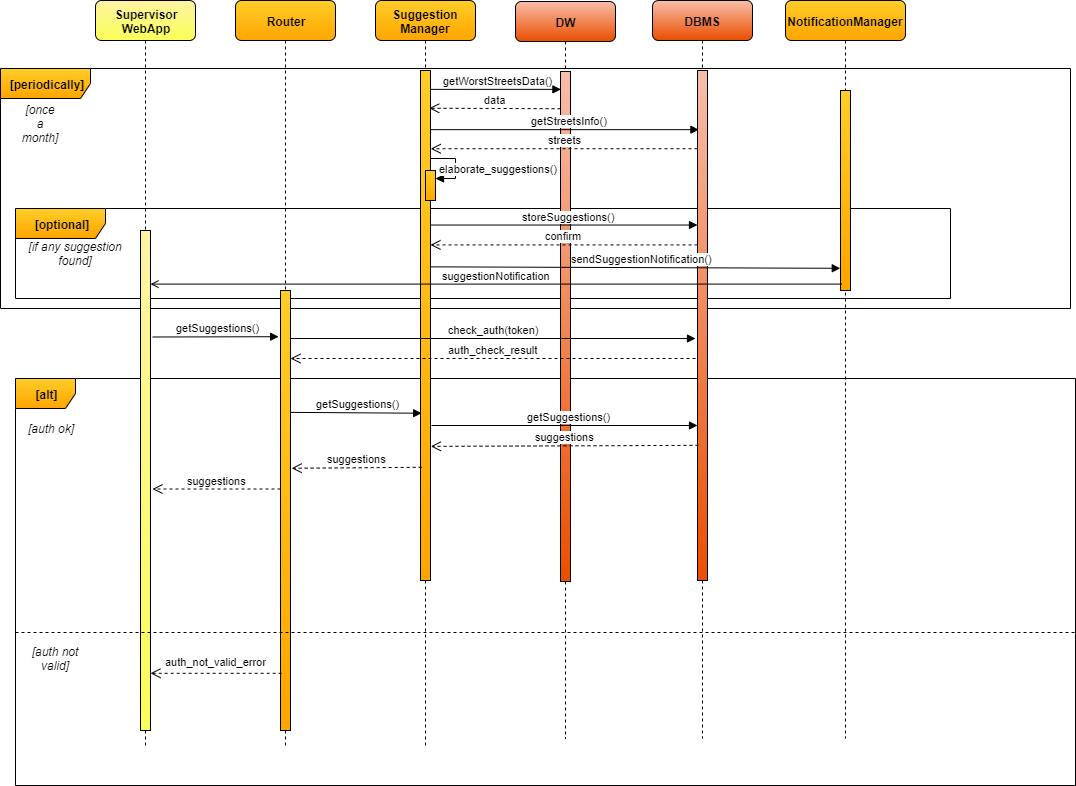
\includegraphics[angle=0, scale=0.65]{ArchSequenceSuggestions}
\caption{UML Architectural Sequence Diagram for the \textit{Suggestions}}
\label{fig:seq-suggestions}
\end{figure}

\end{landscape}
\restoregeometry

In the sequence diagram of figure \ref{fig:seq-sendReport} it has assumed that the \textit{getCity} request to the municipality API returns a city for which the \textit{SafeStreets service} is active. In effect the mobile app should not allow the user to send a report for a city in which the system is not active.\\
In the sequence diagram of figure \ref{fig:seq-checkReport} the control for the user authentication is shown for every request, but only the first one presents the \textit{Alternative} choice, for the others, marked with *, it has been assumed a positive answer, for the sake of readability, avoiding to repeat the \textit{Alt} with the error message returned in case of authentication failure. 
A similar assumption has been made for the municipality answer to the ticket emission request, it has been avoided to report the negative answer, for which the agent would be required to retry the request.

\section{Component interfaces}


\section{Selected architectural	styles and patterns}
\section{Other design decisions}
\subsection{Consistency and update strategies among replicas}
In this application,  we need a client-centric consistency among replicas because end users (and therefore application servers that act as clients towards the DataServers) don't always connect to the same DataServer, due to the presence of the load balancer. Every DataServer can respond to a request to read or write data so we use an active replication protocol. In particular we exploit leaderless replication in which the decision on the value to read and the write to perform is decided by all the replicas or at least a quorum of them. The type of chosen consistency model  is the "read your writes": the effect of a write operation by a process on a data item x will always be seen by a successive read operation on x by the same process. 
Concerning the update propagation we opted for propagating a notification of the operation, assuming that there will be more writes than reads.  The propagation strategy chosen is the Gossiping strategy: when a replica is updated then it just propagates that update to all the nodes that it knows; if a replica receives an update that it has already received then the probability of propagating that information is decreased on that replica. 

\chapter{User interface design}

\chapter{Requirements Traceability}

In this section is shown how the requirements are actually ensured and what components actually ensure them. It's worth to notice that for the sake of simplicity the Router has been ignored but it's always involved when dealing with a request coming from one of the clients. 
In table ref? to highlight for each component what requirements it ensures.
\begin{table}[H]  
  \centering
  \begin{tabular}{|c|c|}
    \cline{1-2}
   	\rule{0pt}{10pt} 
   	\begin{large}
    \textbf{Component} 
    \end{large}&\begin{large}
    \textbf{Requirements} 
    \end{large}\\  \hline
    User Mobile App &  R1, R4, R5, R6, R7, R8, R9, R10, R28, R29, R30, R33, R34, R35 \\ \hline
    MunicipalityAgent Web App & R20, R24, R26 \\ \hline
    MunicipalitySupervisor Web App & R36, R37, R38, R39 \\ \hline
    AccessManager & R1, R2, R3, R25, R26, R38, R39 \\ \hline
    ReportManager & R11, R12, R13, R14, R15, R16, R18, R19, \\ \hline
    SuggestionManager & R42 \\ \hline
    StatisticsManager & R30, R32, R36 \\ \hline
    NotifcationManager & R19, R42 \\ \hline
    DataCollectionManager & R31 \\ \hline
    DataWareHouse & R27, R31, R32, R36, R40, R41, R42 \\ \hline
    
  \end{tabular}
  \caption{Correspondence between goals and world and shared phenoma}
\end{table}
In the following lines is explained how the requirements are provided by the components:
\begin{enumerate}[start=1,label={[R\arabic*]}]
\item The system must allow people to register to it providing personal data (name, surname, birthdate, identity card number, fiscal code) and selecting a username and a password: This requirement is provided by the \textbf{AccessManager} and the \textbf{User Mobile App} components. The \textbf{User Mobile App} allows the user to fill blank spaces with username and password and the \textbf{AccessManager} handles requests of registration from the client.
\item The system must verify the correctness of the provided personal data of a registered user checking them from the identity card number, blocking the registration if they are not correct: the \textbf{AccessManager} checks the received data from the Client and checks them calling the \textbf{munipality API services} that actually possesses sensible data of the users. 
\item The system must allow registered users to login through their username and password: this requirement is provided by the AccessManager (AuthoritiesLogin and CitizenLogin components) that handles the requests of login from the user. 
\item The system must allow logged user to fill a report violation form: this requirement is fulfilled by the User Mobile App comonent that allows user to choose the "Report a violation" feature.
\item The system must let the user select the type of violation detected: the requirement is fulfilled by the User Mobile App component, showing an empty space to fill with the type of violation detected in the report a violation process.
\item The system must allow the user to insert the license plate in a violation report:  the requirement is fulfilled by the User Mobile App component, showing an empty space to fill with the license plate of the car that committed the violation in the report a violation process.
\item While reporting the violation, the system must allow users to take one or more pictures of the potential violation: the requirement is fulfilled by the User Mobile App component, allowing user to click on the "Take a picture" button.
\item The system must not allow users to choose pictures not taken in the moment of the report: this requirement is guaranteed by the User Mobile App by not allowing client to just pick some random picture from his local storage.
\item The system must collect the current position of the user, using GPS: the User Mobile App component ensures this requirement by taking the current position of the User using GPS location.
\item The system must allow user to confirm or delete the current report: the User Mobile App component ensures this requirement by either sending the report for a check through the "confirm" button or deleting the current report clicking on the back button.
\item After confirmation, the system must add the current date and time to the report: the ReportManager actually takes the requests from the client and attaches to them the current time and date taken from the application server internal clock.
\item The system must store confirmed report: the ReportManager is responsible for this requirement, calling the DataServer to actually store the report.
\item The system must check reports to try to find if the pictures of the violations have been modified: the ReportManager manages to check if the pictures are fake or not or have been modified.
\item The system must try to find, according to the GPS position of the user and the pictures sent, if the position is fake or not: the ReportManager ensures this requirement by running an algorithm to define if the position is correct or not. 
\item The system must discard the report if it has been recognized as fake according to the previous requirements (R13-R14): the ReportManager is in charge of this, deleting the report if recognized as fake.
\item The system must try to automatically recognize the license plate in the photo, possibly with the help of the value inserted by the user: the ReportManager is in charge of this , running an algorithm for text recognition in the picture(s).
\item ????? The system must store into stable memory the reported violation if correct (i.e. not recognized as fake). ??????
\item The involved municipality must be calculated considering in which city the reported violation has been found, based on the GPS position of the user that has sent the report: the reportManager provides this requirement by asking the Maps Service the municipality associated to the position of the user.
\item The system must send the reported violations to the involved municipality: the ReportManager and the the NotificationManager are responsible for this. After having saved it, the ReportManager sends the report to the NotificationManager that forwards it to the involved municipality.
\item The system must allow an agent to see the reports for its municipality, checking them in order of arrival: The MunicipalityAgent Web app component is responsible for this, showing on screen the reports in order of arrival.
\item The system must allow an agent to issue a traffic ticket to a certain person (i.e. license plate) through the correspondent municipality service:
\item The system must allow an agent to put on hold a violation report if it needs to be checked in person: The MunicipalityAgent Web App ensures this by shwoing the possibility of putting a report on hold while checking it.
\item The system must allow an agent to discard a violation if it has been verified as fake or it cannot be verified (the vehicle is not there anymore) or it is a duplicated report.??
\item The system must allow an agent to retrieve the data of the author of a violation report: the MunicipalityAgent Web App asks to the Municipality API data about the author of the report. 
\item The system must allow an agent to create an account, asking the municipality services to verify its identity: the AccessManager is responsible for this, asking the Municipality API to check the identity of the agent.
\item The system must allow an agent to login, inserting its username and password: Municipality Web App and AccessManager are responsible for this. The MunicipalityAgent Web App allows agents to insert data, while AccessManager checks if they are correct.
\item The system must mine this information from the reported violations: the DataWareHouse is responsible for this, performing datamining on reports stored in the DataBase of the application.
\item The system must allow the users (even if not authenticated) to select the see information for a city. The user can choose either the city where he is, using the GPS position, or an arbitrary selected location. The User Mobile App component ensures this requirement by allowing user to choose the city he wants.
\item The system must allow the user to select information about streets or areas in the city selected and to specify if he wants information for a specific street or area or a classification of streets or areas. The Mobile Web App is responsible for this requirement by allowing user to choose the area or street he wants.
\item The system must show the the data corresponding to the selection of [R29]: the User Mobile App and Statisticsmanager components are responsible for this requirement; the StatisticsManager contacts the MapAPI to provide an image for the city/area/street selected. This image is then shown by the Mobile App component to the user.
\item The system must take information about accidents and tickets from the municipality: this requirement is ensured by the DataCollectionManager that periodically queries the Municipality API to retrieve new informations and saves them on the DataWareHouse.
\item The system must use this information to build statistics, crossing them with reported violations: the StatisticsManager and the DataWareHouse component ensure this requirement; the DataWareHouse components build statistics exploiting dataMining techniques
\item The system must not allow common users to see confidential data about other people: The User Mobile App component is in charge for this requirement by showing only data that does not violate privacy.This requirement is also guaranteed by a subcomponent in the Router (i.e. AuthChecker) to check if a request made by a specific client is valid or not.
\item The system must allow the user to choose a topic: areas or streets with most accidents, areas or streets with the highest number of traffic tickets issued, areas or streets where there have been the best improvements, information for a specific area or street. The User Mobile App iprovides this requirement by allowing user to choose the topic is interested into.
\item The system must show to the user the information about the topic selected according to [R34]: The User Mobile App component ensures this requirement by showing as an image the topic requested to the user.
\item The system must allow authenticated supervisors to retrieve information about the vehicles with the highest number of violations in a selected area or street: the MunicipalitySupervisor Web App allows supervisors to select the statistics they want; the Statistics;anager asks the the DataWareHouse the type of Data requested by the User.
%\item {[R37]}	\label{R37}The system must allow supervisors to see what areas or streets has seen the best improvements in the ticket emissions.
\item The system must allow supervisors to access only information about their own municipality: the MunicipalitySupervisor Web App  is responsible for this, allowing supervisor to only check Statistics and suggestions about his city. This requirement is also guaranteed by a subcomponent in the Router (i.e. AuthChecker) to check if a request made by a specific client is valid or not.
\item The system must allow a supervisor to create an account, asking the municipality services to verify its identity: the AccessManager and the MunicipalitySupervisor Web App are responsible for this requirement. the accessManager receives the request and ask the MunicipalityAPI to check if the inserted identity is correct.
\item The system must allow a supervisor to login, inserting its username and password: The MunicipalitySupervisor Web App and the AccessManager are responsible for the requirement. The MunicipalitySupervisor WebApp allows supervisor to enter his username and password and forwards the request to the AccessManager that handles it asking the DataServer if the data inserted is correct.
\item The system must take information about accidents, tickets and street networks (bike lanes, sidewalks, parking areas,…) from the municipality, exploiting the municipality services: the DataWareHouse component. ??'
\item The system must elaborate this information, combined with reports information, and try to find possible solutions for problems: the DataWareHouse component is responsible for this requirement trying to aggregate data coming from the Databases concerning reports, issued traffic tickets and accidents.
\item The system must notify the municipality about new possible interventions: the NotificationManager the DataWareHouse and SuggestionManager components are responsible for this requirement: the DataWareHouse component forwards the new intervention to the SuggestionManager that forwards it to NotificationManager that sends it to  the involved municipality.

\end{enumerate}

\chapter{Implementation, integration and test plan}

\chapter{Effort spent}

\begin{table}[H]
\centering
Nicola Rosetti \\
%\begin{tabular}{lll}
\begin{tabular}{p{2cm}p{1.5cm}p{7cm}}
\toprule
\textit{Date} & \textit{Hour} & \textit{Section} \\ \midrule
17-10-2019 & 1.5 h* & Component and high-level architecture analysis \\ \midrule
\bottomrule
\end{tabular}
\caption[Nicola Rosetti's effort table]{}
\end{table}


\vspace*{1 cm}
\begin{table}[H]
\centering
Simone Sartoni \\
\begin{tabular}{p{2cm}p{1.5cm}p{7cm}}
\toprule
\textit{Date} & \textit{Hour} & \textit{Section} \\ \midrule
18-11-2019 & 1 h* & Componenst and high-level architecture analysis \\ \midrule
24-11-2019 & 4 h &  System architecture diagram and deployment diagram\\ \midrule
27-11-2019 & 1.5 h & Update deployment diagram, requirements traceability revision and Requirements Traceability Matrix creation \\ \midrule
28-11-2019 & 1 h & Requirements Traceability Matrix update \\ \midrule

\bottomrule
\end{tabular}
\caption[Simone Sartoni's effort table]{}
\end{table}
\vspace*{1 cm}
\begin{table}[H]
\centering
Vittorio Torri \\
\begin{tabular}{p{2cm}p{1.5cm}p{7cm}}
\toprule
\textit{Date} & \textit{Hour} & \textit{Section} \\ \midrule
18-11-2019 & 1 h* & Componenst and high-level architecture analysis \\ \midrule
21-11-2019 & 1 h  & Components diagram \\ \midrule
22-11-2019 & 0.5 h & Components diagrams \\ \midrule
23-11-2019 & 1.5 h & Components diagrams and components view\\ \midrule
24-11-2019 & 2 h & Sequence diagrams and components view \\ \midrule
26-11-2019 & 1 h & Sequence diagrams \\ \midrule
27-11-2019 & 1 h & Sequence diagrams \\ \midrule
28-11-2019 & 1 h* & RASD Update \\ \midrule
28-11-2019 & 1 h & Sequence Diagram \\ \midrule
\bottomrule
\end{tabular}
\caption[Vittorio Torri's effort table]{}
\end{table}
\textit{* Group work}

\chapter{References}


\end{document}
